\documentclass[11pt]{article}

\usepackage[margin=1in]{geometry}
\usepackage{setspace}
\onehalfspacing
\usepackage{graphicx}
\graphicspath{report_images/}
\usepackage{appendix}
\usepackage{listings}
\usepackage{float}
\usepackage{multirow}
\usepackage{amsthm}
% The next three lines make the table and figure numbers also include section number
\usepackage{chngcntr}
\counterwithin{table}{section}
\counterwithin{figure}{section}
% Needed to make titling page without a page number
\usepackage{titling}

% DOCUMENT INFORMATION =================================================
\font\titleFont=cmr12 at 11pt
\title {{\titleFont ECEN 429: Introduction to Digital Systems Design Laboratory \\ North Carolina Agricultural and Technical State University \\ Department of Electrical and Computer Engineering}} % Declare Title
\author{\titleFont Reporter: Chris Cannon\\ \titleFont Partner: Nikiyah Beulah} % Declare authors
\date{\titleFont March 1, 2018}
% ======================================================================

\begin{document}

\begin{titlingpage}
\maketitle
\begin{center}
	Lab 7
\end{center}
\end{titlingpage}

\section{Introduction}
This lab tests our 

\section{Background, Design Solution, and Results}

\subsection{Problem 1 }

\subsubsection{Background}


\subsubsection{Design Solution}


\begin{table}[H]
\begin{center}
\begin{tabular}{| l | l | l |}
	\hline
	Bit & Label & Port \\ \hline
	FastClock & LED 0 & U16 \\ \hline
	MediumClock & LED 1 & E19 \\ \hline
	SlowClock & LED 2 & U19 \\ \hline
	led0 & LED 15 & L1 \\ \hline
\end{tabular}
\caption{\label{tab:clockDivider_input_Ports}Input port assignments for Clock Divider.}
\end{center}
\end{table}

\begin{table}[H]
\begin{center}
\begin{tabular}{| l | l | l |}
	\hline
	Bit & Label & Port \\ \hline
	clk & Clock & W5 \\ \hline
	starttimer & Switch 0 & V17 \\ \hline
\end{tabular}
\caption{\label{tab:clockDivider_output_Ports}Output port assignments for Clock Divider.}
\end{center}
\end{table}

\subsubsection{Results}


\subsection{Problem 2 }

\subsubsection{Background}

\subsubsection{Design Solution}


\subsubsection{Results}

\subsection{Problem 3}

\subsubsection{Background}


\subsubsection{Design Solution}


\subsubsection{Results}


\section{Conclusion}


\pagebreak

\textbf{Appendices}

\begin{appendices}

\section{Problem 1 VHDL Code}

\begin{lstlisting}[language=VHDL]
library IEEE;
use IEEE.STD_LOGIC_1164.ALL;

entity bitwise_and is port(a, b : in STD_LOGIC_VECTOR(1 downto 0); v: out STD_LOGIC_VECTOR(1 downto 0));
end entity bitwise_and;

architecture and_arch of bitwise_and is
begin
    v <= a and b;
end architecture and_arch;

library IEEE;
use IEEE.STD_LOGIC_1164.ALL;

entity bitwise_or is port(c, d : in STD_LOGIC_VECTOR(1 downto 0); x: out STD_LOGIC_VECTOR(1 downto 0));
end entity bitwise_or;

architecture or_arch of bitwise_or is
begin
  x <= c or d;
end architecture or_arch;

library IEEE;
use IEEE.STD_LOGIC_1164.ALL;

entity bitwise_lsr is port(e, f : in STD_LOGIC_VECTOR(1 downto 0); y : out STD_LOGIC_VECTOR(1 downto 0));
end bitwise_lsr;

architecture lsr_arch of bitwise_lsr is
begin
    process(e, f)
    begin
        case f is
        when "00" =>
            y <= e;
        when "01" =>
            if(e = "00") then y <= "00";
            elsif(e = "01") then y <= "00";
            else y <= "01";
            end if;
        when others =>
            y <= "00";
        end case;
     end process;
end lsr_arch;

library IEEE;
use IEEE.STD_LOGIC_1164.ALL;

entity bitwise_lsl is port(g, h : in STD_LOGIC_VECTOR(1 DOWNTO 0); z : out STD_LOGIC_VECTOR(1 downto 0));
end bitwise_lsl;

architecture lsl_arch of bitwise_lsl is
begin
    process(g, h)
    begin
        case h is
        when "00" =>
            z <= g;
        when "01" =>
            if(g = "11") then z <= "10";
            elsif(g = "01") then z <="10";
            else z <= "00";
            end if;
        when others =>
            z <= "00";
        end case;
    end process;
end lsl_arch;

library IEEE;
use IEEE.STD_LOGIC_1164.ALL;

entity ArithmeticLogicUnit is
    Port ( in1 : in STD_LOGIC_VECTOR(1 downto 0);
           in2 : in STD_LOGIC_VECTOR(1 downto 0);
           sel : in STD_LOGIC_VECTOR(1 downto 0);
           output : out STD_LOGIC_VECTOR(1 downto 0));
end ArithmeticLogicUnit;

architecture Behavioral of ArithmeticLogicUnit is
component bitwise_and is port(a, b : in STD_LOGIC_VECTOR(1 downto 0); v : out STD_LOGIC_VECTOR(1 downto 0));
end component bitwise_and;

component bitwise_or is port(c, d : in STD_LOGIC_VECTOR(1 downto 0); x : out STD_LOGIC_VECTOR(1 downto 0));
end component bitwise_or;

component bitwise_lsr is port(e, f : in STD_LOGIC_VECTOR(1 downto 0); y : out STD_LOGIC_VECTOR(1 downto 0));
end component bitwise_lsr;

component bitwise_lsl is port(g, h : in STD_LOGIC_VECTOR(1 DOWNTO 0); z : out STD_LOGIC_VECTOR(1 downto 0));
end component bitwise_lsl;

signal and_output : STD_LOGIC_VECTOR(1 downto 0);
signal or_output : STD_LOGIC_VECTOR(1 downto 0);
signal lsr_output : STD_LOGIC_VECTOR(1 downto 0);
signal lsl_output : STD_LOGIC_VECTOR(1 downto 0);

begin
    and_comp : bitwise_and port map(in1, in2, and_output);
    or_comp : bitwise_or port map(in1, in2, or_output);
    lsr_comp : bitwise_lsr port map(in1, in2, lsr_output);
    lsl_comp : bitwise_lsl port map(in1, in2, lsl_output);
    
    process(sel)
    begin
        case sel is
            when "00" =>
                output <= and_output;
            when "01" =>
                output <= or_output;
            when "10" =>
                output <= lsr_output;
            when "11" =>
                output <= lsl_output;
        end case;
    end process;                

end Behavioral;
\end{lstlisting}

\section{Problem 1 Constraints File}
\begin{center}
\begin{figure}[H]
	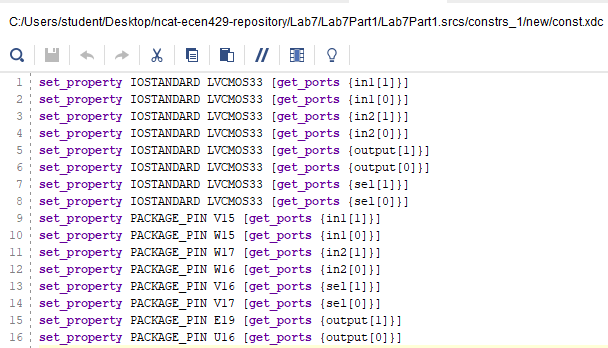
\includegraphics[scale=1]{./images/Lab7Part1Const.png}
	\caption{\label{fig:Prob1Const}Constraints file for Problem 1.}
\end{figure}
\end{center}

\section{Problem 2 VHDL Code}
\begin{lstlisting}[language=VHDL]
library IEEE;
use IEEE.STD_LOGIC_1164.ALL;

entity FSM is
    Port ( clk : in STD_LOGIC;
           enable : in STD_LOGIC;
           reset : in STD_LOGIC;
           output_sel : out STD_LOGIC_VECTOR(1 downto 0);
           clock_led : out STD_LOGIC);
end FSM;

architecture Behavioral of FSM is
component Clockdivider is 
          Port (clk : in std_logic;
          start_timer : in std_logic;
	      FastClock,MediumClock,SlowClock, led0 : out std_logic);
end component Clockdivider;

signal fastclocksig :STD_LOGIC;
signal medclocksig :STD_LOGIC;
signal slowclocksig :STD_LOGIC;
signal current_state : STD_LOGIC_VECTOR(1 downto 0) := "00";

begin
    clockDiv : Clockdivider port map(clk, reset, fastclocksig, medclocksig, slowclocksig, clock_led);
    
    process(slowclocksig, reset)
    begin
        if(reset = '1') then
            current_state <= "00";
            output_sel <= "00";
        end if;
        if(slowclocksig'event and (slowclocksig = '1')) then
            if(enable = '1') then
            case current_state is
                when "00" =>
                    current_state <= "01";
                    output_sel <= "01";
                when "01" =>
                    current_state <= "10";
                    output_sel <= "10";
                when "10" =>
                    current_state <= "11";
                    output_sel <= "11";
                when "11" =>
                    current_state <= "00";
                    output_sel <= "00";
            end case;
            else
                current_state <= "00";
                output_sel <= "00";
            end if;
        end if;
    end process;
    
    output_sel <= current_state;
end Behavioral;
\end{lstlisting}

\section{Problem 2 Constraints File}
\begin{center}
\begin{figure}[H]
	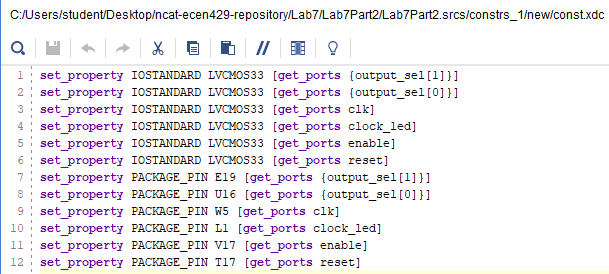
\includegraphics[scale=1]{./images/Lab7Part2Const.png}
	\caption{\label{fig:Prob1Const}Constraints file for Problem 2.}
\end{figure}
\end{center}

\section{Problem 3 VHDL Code}
\begin{lstlisting}[language=VHDL]
library IEEE;
use IEEE.STD_LOGIC_1164.ALL;

entity TopLevelDesign is
    Port ( input1 : in STD_LOGIC_VECTOR(1 downto 0);
           input2 : in STD_LOGIC_VECTOR(1 downto 0);
           clk : in STD_LOGIC;
           enable : in STD_LOGIC;
           reset : in STD_LOGIC;
           output : out STD_LOGIC_VECTOR(1 downto 0);
           clock_led : out STD_LOGIC;
           operation : out STD_LOGIC_VECTOR(1 downto 0));
end TopLevelDesign;

architecture Behavioral of TopLevelDesign is
component FSM is
    Port ( clk : in STD_LOGIC;
           enable : in STD_LOGIC;
           reset : in STD_LOGIC;
           output_sel : out STD_LOGIC_VECTOR(1 downto 0);
           clock_led : out STD_LOGIC);
end component FSM;

component ArithmeticLogicUnit is
    Port ( in1 : in STD_LOGIC_VECTOR(1 downto 0);
           in2 : in STD_LOGIC_VECTOR(1 downto 0);
           sel : in STD_LOGIC_VECTOR(1 downto 0);
           output : out STD_LOGIC_VECTOR(1 downto 0));
end component ArithmeticLogicUnit;

signal select_signal : STD_LOGIC_VECTOR(1 downto 0);

begin
    stateMachine : FSM port map(clk, enable, reset, select_signal, clock_led);
    logicUnit : ArithmeticLogicUnit port map(input1, input2, select_signal, output);
    operation <= select_signal;
end Behavioral;
\end{lstlisting}

\section{Problem 3 Constraints File}
\begin{center}
\begin{figure}[H]
	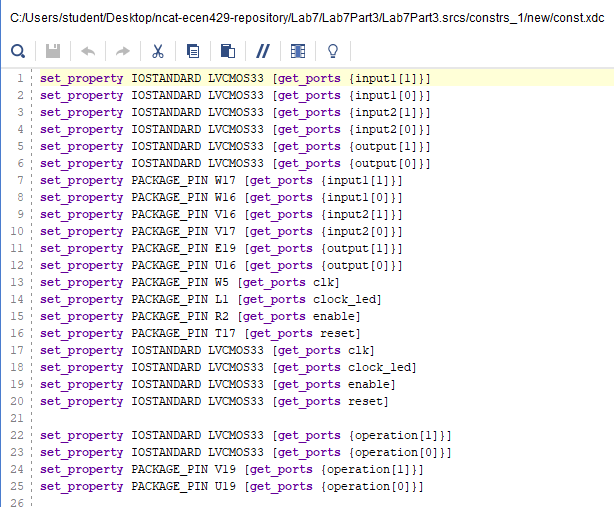
\includegraphics[scale=1]{./images/Lab7Part3Const.png}
	\caption{\label{fig:Prob1Const}Constraints file for Problem 3.}
\end{figure}
\end{center}

\end{appendices}
\end{document}
